\documentclass[a4paper]{article}
\usepackage{tikz}
\usetikzlibrary{arrows,backgrounds,positioning,calc,fit,shapes.geometric,decorations.pathreplacing,decorations.markings}
\usepackage{geometry}
\usepackage{graphicx}
\usepackage{natbib}
\usepackage{amsmath}
\usepackage{amssymb}
\usepackage{amsthm}
\usepackage{paralist}
\usepackage{epstopdf}
\usepackage{tabularx}
\usepackage{longtable}
\usepackage{multirow}
\usepackage{multicol}
\usepackage[hidelinks]{hyperref}
\usepackage{fancyvrb}
\usepackage{algorithm}
\usepackage{algorithmic}
\usepackage{float}
\usepackage{paralist}
%\usepackage[svgname]{xcolor}
\usepackage{enumerate}
\usepackage{array}
\usepackage{times}
\usepackage{url}
\usepackage{fancyhdr}
\usepackage{comment}
\usepackage{environ}
\usepackage{times}
\usepackage{textcomp}
\usepackage{caption}
\usepackage{bbm}


\urlstyle{rm}

\setlength\parindent{0pt} % Removes all indentation from paragraphs
\theoremstyle{definition}
\newtheorem{definition}{Definition}[]
\newtheorem{conjecture}{Conjecture}[]
\newtheorem{example}{Example}[]
\newtheorem{theorem}{Theorem}[]
\newtheorem{lemma}{Lemma}
\newtheorem{proposition}{Proposition}
\newtheorem{corollary}{Corollary}

\floatname{algorithm}{Procedure}
\renewcommand{\algorithmicrequire}{\textbf{Input:}}
\renewcommand{\algorithmicensure}{\textbf{Output:}}
\newcommand{\abs}[1]{\lvert#1\rvert}
\newcommand{\norm}[1]{\lVert#1\rVert}
\newcommand{\RR}{\mathbb{R}}
\newcommand{\CC}{\mathbb{C}}
\newcommand{\Nat}{\mathbb{N}}
\newcommand{\br}[1]{\{#1\}}
\DeclareMathOperator*{\argmin}{arg\,min}
\DeclareMathOperator*{\argmax}{arg\,max}
\renewcommand{\qedsymbol}{$\blacksquare$}

\definecolor{dkgreen}{rgb}{0,0.6,0}
\definecolor{gray}{rgb}{0.5,0.5,0.5}
\definecolor{mauve}{rgb}{0.58,0,0.82}

\definecolor{C0}{HTML}{1F77B4}
\definecolor{C1}{HTML}{FF7F0E}
\definecolor{C2}{HTML}{2ca02c}
\definecolor{C3}{HTML}{d62728}
\definecolor{C4}{HTML}{9467bd}
\definecolor{C5}{HTML}{8c564b}
\definecolor{C6}{HTML}{e377c2}
\definecolor{C7}{HTML}{7F7F7F}
\definecolor{C8}{HTML}{bcbd22}
\definecolor{C9}{HTML}{17BECF}

\newcommand{\Var}{\mathrm{Var}}
\newcommand{\Cov}{\mathrm{Cov}}
\newcommand{\sgn}{\mathrm{sgn}}

\newcommand{\vc}[1]{\boldsymbol{#1}}
\newcommand{\xv}{\vc{x}}
\newcommand{\Sigmav}{\vc{\Sigma}}
\newcommand{\alphav}{\vc{\alpha}}
\newcommand{\muv}{\vc{\mu}}

\newcommand{\red}[1]{\textcolor{red}{#1}}

\def\x{\mathbf x}
\def\y{\mathbf y}
\def\w{\mathbf w}
\def\v{\mathbf v}
\def\E{\mathbb E}
\def\R{\mathbb R}
\def\V{\mathbb V}
\def\ind{\mathbbm 1}

% TO SHOW SOLUTIONS, include following (else comment out):
\newenvironment{soln}{
    \leavevmode\color{blue}\ignorespaces
}{}


\hypersetup{
%    colorlinks,
    linkcolor={red!50!black},
    citecolor={blue!50!black},
    urlcolor={blue!80!black}
}

\geometry{
  top=1in,            % <-- you want to adjust this
  inner=1in,
  outer=1in,
  bottom=1in,
  headheight=3em,       % <-- and this
  headsep=2em,          % <-- and this
  footskip=3em,
}


\pagestyle{fancyplain}
\lhead{\fancyplain{}{Homework 7}}
\rhead{\fancyplain{}{CS 760 Machine Learning}}
\cfoot{\thepage}

\title{\textsc{Homework 7}} % Title

%%% NOTE:  Replace 'NAME HERE' etc., and delete any "\red{}" wrappers (so it won't show up as red)

\author{
\red{Daniel Szabo} \\
\red{9074762189}\\
} 

\date{}

\begin{document}

\maketitle 


\textbf{Instructions:} 
There is no need to submit the latex source or any code.
You can choose any programming language, as long as you implement the algorithm from scratch. Use this latex file as a template to develop your homework.
Submit your homework on time as a single pdf file to Canvas.
Please check Piazza for updates about the homework.\\

\section{Chow-Liu Algorithm [100 pts]}
Suppose we wish to construct a directed graphical model for 3 features $X$, $Y$, and $Z$ using the Chow-Liu algorithm. We are given data from 100 independent experiments where each feature is binary and takes value $T$ or $F$. Below is a table summarizing the observations of the experiment:

\begin{table}[H]
        \centering
                \begin{tabular}{cccc}
                           $X$ & $Y$ & $Z$ & Count \\
                                \hline
                                T & T & T & 36 \\
                                \hline
                                T & T & F & 4 \\
                                \hline
                                T & F & T & 2 \\
                                \hline
                                T & F & F & 8 \\
                                \hline
                                F & T & T & 9 \\
                                \hline
                                F & T & F & 1 \\
                                \hline
                                F & F & T & 8 \\
                                \hline
                                F & F & F & 32 \\
                                \hline
                \end{tabular}
\end{table}

\begin{enumerate}
	\item Compute the mutual information $I(X, Y)$ based on the frequencies observed in the data. (20 pts)
	
	\begin{soln}
		\begin{align*}
			I(X,Y) &= H(X) - H(X|Y) = -(.5\log .5 + .5\log .5) + (.5 (.8\log .8 + .2\log .2) + .5 (.2\log .2 + .8\log .8))\\
			&= 0.278072...
		\end{align*}
	\end{soln}

	\item Compute the mutual information $I(X, Z)$ based on the frequencies observed in the data. (20 pts)
	
	\begin{soln}
		\begin{align*}
			I(X,Z) &= H(X) - H(X|Y) = 1 + (.55 (\frac{38}{55}\log \frac{38}{55} + \frac{17}{55}\log \frac{17}{55}) + .45 (\frac{12}{45}\log \frac{12}{45} + \frac{33}{45}\log \frac{33}{45}))\\
			&= 0.132845...
		\end{align*}
	\end{soln}

	\item Compute the mutual information $I(Z, Y)$ based on the frequencies observed in the data. (20 pts)
	
	\begin{soln}
		\begin{align*}
			I(Z,Y) &= H(Y) - H(Y|Z) = 1 + (.55 (\frac{45}{55}\log \frac{45}{55} + \frac{10}{55}\log \frac{10}{55}) + .45 (\frac{5}{45}\log \frac{5}{45} + \frac{40}{45}\log \frac{40}{45}))\\
			&= 0.397313...
		\end{align*}
	\end{soln}
	
	\item Which undirected edges will be selected by the Chow-Liu algorithm as the maximum spanning tree? (20 pts)
	
	\begin{soln}
		Any two edges would make a spanning tree, so the maximum spanning tree would be the one with the two edges that have the highest mutual information, namely $ (Z,Y) $ and $ (X,Y) $.
	\end{soln}
	
	\item Root your tree at node $X$, assign directions to the selected edges. (20 pts)
	\begin{soln}
		If we have the root at $ X $, the directed edges would be $ (X,Y) $ and $ (Y,Z) $. The graph would look like:
		\begin{figure}[h]
		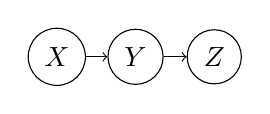
\begin{tikzpicture}
			\node[shape=circle, draw] (X) {$ X $}; \node[shape=circle, draw] (Y) [right of=X] {$ Y $}; \node[shape=circle, draw] (Z) [right of=Y] {$ Z $};
			\path (X) edge[->] (Y);
			\path (Y) edge[->] (Z);
		\end{tikzpicture}
		\end{figure}
	\end{soln}
\end{enumerate}

\end{document}
